\RequirePackage{plautopatch}
\documentclass[aspectratio=169, dvipdfmx, 8pt, notheorems, uplatex]{beamer}
\usepackage{docmute}
\usepackage{mypackage}

\title[]{$\Ainf$増強としてのホモロジカルミラー対称性}
\subtitle{}
\author[第4回 すうがく徒のつどい オンライン]{よの}
\date{2023年9月16日}

\begin{document}
\maketitle

\begin{frame}{目次}
  \tableofcontents
\end{frame}

% \section{加法圏とAbel圏}

% \begin{frame}
%   環上の加群の圏$\Mod(A)$を抽象化した圏でホモロジー代数を展開する. \bigskip

%   \begin{block}{$\Mod(A)$の持つ性質}
%     \begin{enumerate}
%       \item $\hom_{\Mod(A)}(X,Y)$は加法群の構造を持つ.
%       \item $\hom_{\Mod(A)}(X,Y)$は零元を与える零射を持つ. 
%       \item 任意の射は核と余核を持つ.
%       \item 任意の射に対して, 準同型定理が成立する. 
%     \end{enumerate}   
%   \end{block}
% \end{frame}

% \begin{frame}
%   $\Mod(A)$の持つ性質を抽象化して, (前)加法圏やAbel圏を定義する. 

%   \begin{definition}[前加法圏]
%     圏$\C$が次の条件を満たすとき, $\C$を前加法圏(pre-additive category)という. 
%     \begin{itemize}
%       \item 任意の$X,Y \in \C$に対して, $\hom_\C(X,Y)$は加法群
%       \item 合成$\circ$は双線形写像
%     \end{itemize}
%   \end{definition}

%   \begin{definition}[加法圏]
%     前加法圏$\C$が次の条件を満たすとき, $\C$を加法圏(additive category)という. 
%     \begin{itemize}
%       \item $\C$は零対象$0$を持つ.
%       \item $\C$は有限余直和を持つ. 
%     \end{itemize}
%   \end{definition}

%   \begin{example}
%     $\Ab$や$\Mod(A)$は加法圏である. 
%   \end{example}
% \end{frame}

% \begin{frame}
%   加群の複体の定義を抽象化して, 一般の加法圏上で考える.
%   $\C$を加法圏とする.

%   \begin{definition}[複体]
%     $\C$の対象と射の集まり$X = \{X^i,d^i\}_{i \in \bbZ}$
%     \begin{align*}
%       X = \cdots \to X^{i-1} \xrightarrow{d^{i-1}} X^i \xrightarrow{d^i} X^{i+1} \to \cdots
%     \end{align*}
%     が, $d^i \circ d^{i-1} = 0$を満たすとき, $X$を複体(complex)という.
%   \end{definition}

%   \begin{definition}[複体の射]
%     $X,Y$を$\C$の複体とする.
%     $\C$の射の集まり$f = \{f^i : X^i \to Y^i\}_{i \in \bbZ}$が
%     \begin{align*}
%       f^{i+1} \circ d^i_X = d^i_Y \circ f^i
%     \end{align*}
%     を満たすとき, $f$を$X$から$Y$への複体の射(morphism of complexes)という.
%   \end{definition}

%   \begin{definition}[複体の圏]
%     $\C$の複体と複体の射のなす圏を$C(\C)$と表し, 複体の圏(category of comlexes)という. 
%   \end{definition}
% \end{frame}

% \begin{frame}
%   \begin{definition}[Abel圏]
%     加法圏$\C$が次の条件を満たすとき, $\C$をAbel圏(Abelian category)という. 
%     \begin{itemize}
%       \item $\C$の任意の射は核と余核を持つ.
%       \item $\C$の任意の射$f$に対して, 自然な射$\Coim(f) \to \Im(f)$は同型である. 
%     \end{itemize}
%   \end{definition}
% \end{frame}


\section{ホモロジカルミラー対称性とは}

\begin{frame}{ミラー対称性の周辺 \cite{nlab}}
  複素数体上の$3$次元Calabi-Yau多様体$M$に対して, 2種類の$N=2$超(対称性)2次元共形場理論が考えられる.

  ミラー対称性とは次のような予想である. 
  \footnote{
    筆者は物理の話を知らないので, このページは間違ったことを言っている可能性が高いです.
  }

  \begin{conjecture}[ミラー対称性]
    あるCalabi-Yau多様体$M$に対して, Hodge数$h^{1,1}$と$h^{1,2}$を交換する対応$M \mapsto \hat{M}$が存在し, 超共形場理論$\mathrm{SCFT}_A(M)$と$\mathrm{SCFT}_B(\hat{M})$は等価である. 
  \end{conjecture} 

  ミラー対称性が予想である理由として, そもそも超共形場理論の数学的な定式化が存在しないことがある. 
  しかし、このような超共形場理論にはAモデル$A(M)$とBモデル$B(M)$という2つのモデルを関連付けることができる. 
  ミラー対称性は対応$M \mapsto \hat{M}$に対して, このAモデルとBモデルの等価性と表せる. 
  \begin{align*}
    A(M) \cong B(\hat{M}), ~~ B(M) \cong A(\hat{M})
  \end{align*} 

  Kontsevichはこの等価性を圏論の言葉で表し, ホモロジカルミラー対称性と呼んだ. 
  
  \begin{conjecture}[増強としてのホモロジカルミラー対称性]
    Aモデルはシンプレクティック多様体$M$上のLagrangian部分多様体のなすFukaya圏$\Fuk(M)$によって表される.
    また, Bモデルは$\hat{M}$上の連接層の導来圏の増強$D^b_\infty(\coh(\hat{M}))$で表される. 
    \begin{align*}
      \Fuk(M) \cong D^b_\infty(\coh(\hat{M})), ~~ \Fuk(\hat{M}) \cong D^b_\infty(\coh(M))
    \end{align*}
  \end{conjecture}
\end{frame}


\section{復習 : 三角圏}

\begin{frame}{三角圏について}
  \begin{block}{}
    三角圏は複体の導来圏の持つ性質を調べるためにGrothendieckとVerdier \cite{Ver96}により導入された, Abel圏の持つ写像錐とシフトの性質に注目して公理化された圏である.  \bigskip

    一方, 代数的トポロジーの分野で, Puppeが安定ホモトピー圏を調べるために三角圏の公理を考えている.
    よって, 三角圏は複体の導来圏や安定ホモトピー圏を例に持つ. \bigskip

    コホモロジーを取ると情報が落ちるので, 複体のまま取り扱うのが導来圏の哲学である. 
    三角圏の対象は複体に格上げされるが, 射はコホモロジーを取る (つまり, 複体の間の射として鎖写像のみを考え, ホモトピー同値な射は同一視する)ことが後述の不都合の原因である. 
    そのため, 導来圏の構成でホモトピー圏をとる前, 例えばdg圏や$\Ainf$圏の段階で考えようとすることが考えられた. 
    この考えが増強と呼ばれるものであり, ホモロジカルミラー対称性に深くかかわっている. \bigskip

    この節では, 三角圏と三角圏の間の三角関手を定義するのみにとどめるが, 三角圏は様々な応用をもつので興味のある読者は調べてください. \cite{Nak15,Nee01, Nic17} 
  \end{block}
\end{frame}

\begin{frame}{三角圏}
  $\T$を加法圏, $T: \T \to \T$を加法的自己圏同値とする. 
  
  \begin{definition}[三角]
    $\T$の対象$X, Y, Z$と射$u: X \to Y, v: Y \to Z, w: Z \to TX$
    \footnote{
      対象$X$と射$f$に対して, $T(X)$を$TX$, $T(f)$を$Tf$, $T^{-1}(X)$を$-TX$, $T^{-1}(f)$を$-Tf$とあらわす. 
    }
    の組$(X,Y,Z,u,v,w)$からなる次の図式を三角(triangle)という. 
    \[
      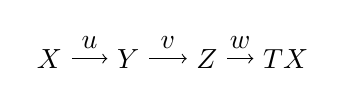
\begin{tikzpicture}[auto,->]
        \node (X) at (0,1) {$X$};
        \node (Y) at (1,1) {$Y$}; 
        \node (Z) at (2,1) {$Z$}; 
        \node (TX) at (3,1) {$TX$};
        \draw (X) -- node {$u$} (Y);
        \draw (Y) -- node {$v$} (Z);
        \draw (Z) -- node {$w$} (TX);
      \end{tikzpicture}
    \]
  \end{definition} 

  \begin{definition}[三角の射]
    $X \xrightarrow{u} Y \xrightarrow{v} Z \xrightarrow{w} TX$と$X' \xrightarrow{u'} Y' \xrightarrow{v'} Z' \xrightarrow{w'} TX'$を完全三角とする. 
    $\T$の射$f: X \to X', g: Y \to Y', h: Z \to Z'$の組$(f,g,h)$であって, 次の図式を可換にするものを三角の射(morphism of triangles)という. 
    \[
      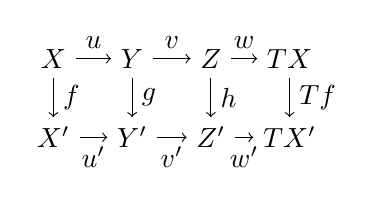
\begin{tikzpicture}[auto,->]
        \node (X') at (0,0) {$X'$};
        \node (Y') at (1,0) {$Y'$}; 
        \node (Z') at (2,0) {$Z'$}; 
        \node (TX') at (3,0) {$TX'$};
        \node (X) at (0,1) {$X$};
        \node (Y) at (1,1) {$Y$}; 
        \node (Z) at (2,1) {$Z$}; 
        \node (TX) at (3,1) {$TX$};
        \draw (X) -- node {$u$} (Y);
        \draw (Y) -- node {$v$} (Z);
        \draw (Z) -- node {$w$} (TX);
        \draw (X') -- node[swap] {$u'$} (Y');
        \draw (Y') -- node[swap] {$v'$} (Z');
        \draw (Z') -- node[swap] {$w'$} (TX');
        \draw (X) -- node {$f$} (X');
        \draw (Y) -- node {$g$} (Y');
        \draw (Z) -- node {$h$} (Z');
        \draw (TX) -- node {$Tf$} (TX');
      \end{tikzpicture}
    \]
  \end{definition}
\end{frame}

\begin{frame}
  \begin{definition}[三角圏]
    三角系列の圏の充満部分圏を$\Delta$と表し, $\Delta$に属する三角を完全三角(distinguished triangle)という. 
    組$(\T, T, \Delta)$が次の条件を満たすとき, $(\T,T,\Delta)$を三角圏(triangulated category), $T$をシフト関手(shift functor)という. 
    \begin{description}
      \item[(TR1)] $\Delta$は同型で閉じる.
      \item[(TR2)] 任意の$X \in \T$に対して, 
      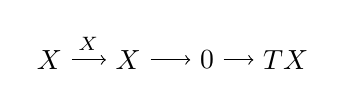
\begin{tikzpicture}[auto,->]
        \node (X) at (0,1) {$X$};
        \node (Y) at (1,1) {$X$}; 
        \node (Z) at (2,1) {$0$}; 
        \node (TX) at (3,1) {$TX$};
        \draw (X) -- node {$\id_X$} (Y);
        \draw (Y) -- (Z);
        \draw (Z) -- (TX);
      \end{tikzpicture}
      は完全三角
      \item[(TR3)] 任意の射$f: X \to Y$に対して, ある$Z \in \T$が存在して, 
      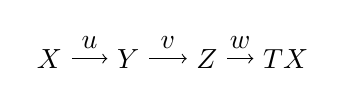
\begin{tikzpicture}[auto,->]
        \node (X) at (0,1) {$X$};
        \node (Y) at (1,1) {$Y$}; 
        \node (Z) at (2,1) {$Z$}; 
        \node (TX) at (3,1) {$TX$};
        \draw (X) -- node {$u$} (Y);
        \draw (Y) -- node {$v$} (Z);
        \draw (Z) -- node {$w$} (TX);
      \end{tikzpicture}
      は完全三角
      \item[(TR4)] 
      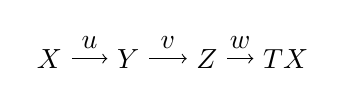
\begin{tikzpicture}[auto,->]
        \node (X) at (0,1) {$X$};
        \node (Y) at (1,1) {$Y$}; 
        \node (Z) at (2,1) {$Z$}; 
        \node (TX) at (3,1) {$TX$};
        \draw (X) -- node {$u$} (Y);
        \draw (Y) -- node {$v$} (Z);
        \draw (Z) -- node {$w$} (TX);
      \end{tikzpicture}
      が完全であることと, 
      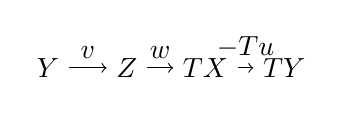
\begin{tikzpicture}[auto,->]
        \node (Y) at (0,1) {$Y$};
        \node (Z) at (1,1) {$Z$}; 
        \node (TX) at (2,1) {$TX$}; 
        \node (TY) at (3,1) {$TY$};
        \draw (Y) -- node {$v$} (Z);
        \draw (Z) -- node {$w$} (TX);
        \draw (TX) -- node {$-Tu$} (TY);
      \end{tikzpicture}
      が完全であることは同値である. 
      \item[(TR5)] 2つの完全三角と射$f: X \to X', g: Y \to Y'$が次の図式を可換にするとき, ある射$h: Z \to Z'$が存在して, 次の図式は可換である. 
      \[
        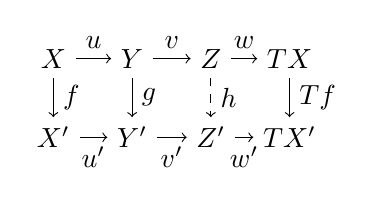
\begin{tikzpicture}[auto,->]
          \node (X') at (0,0) {$X'$};
          \node (Y') at (1,0) {$Y'$}; 
          \node (Z') at (2,0) {$Z'$}; 
          \node (TX') at (3,0) {$TX'$};
          \node (X) at (0,1) {$X$};
          \node (Y) at (1,1) {$Y$}; 
          \node (Z) at (2,1) {$Z$}; 
          \node (TX) at (3,1) {$TX$};
          \draw (X) -- node {$u$} (Y);
          \draw (Y) -- node {$v$} (Z);
          \draw (Z) -- node {$w$} (TX);
          \draw (X') -- node[swap] {$u'$} (Y');
          \draw (Y') -- node[swap] {$v'$} (Z');
          \draw (Z') -- node[swap] {$w'$} (TX');
          \draw (X) -- node {$f$} (X');
          \draw (Y) -- node {$g$} (Y');
          \draw[dashed] (Z) -- node {$h$} (Z');
          \draw (TX) -- node {$Tf$} (TX');
        \end{tikzpicture}
      \]
      \item[(TR6)] 八面体公理(省略)
    \end{description}
  \end{definition}
\end{frame}

\begin{frame}
  三角圏の間の三角関手を定義する. 

  \begin{definition}[三角関手]
    $\T, \T'$を三角圏とする. 
    加法関手$F: \T \to \T'$が次の条件を満たすとき, $F$を三角関手(triangulated functor)という.
    \begin{itemize}
      \item 自然同型$\varphi: F \circ T \simeq T' \circ F$が存在する. 
      \item $\T$の任意の完全三角
      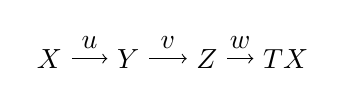
\begin{tikzpicture}[auto,->]
        \node (X) at (0,1) {$X$};
        \node (Y) at (1,1) {$Y$}; 
        \node (Z) at (2,1) {$Z$}; 
        \node (TX) at (3,1) {$TX$};
        \draw (X) -- node {$u$} (Y);
        \draw (Y) -- node {$v$} (Z);
        \draw (Z) -- node {$w$} (TX);
      \end{tikzpicture}
      に対して, 
      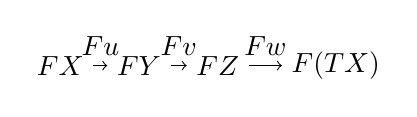
\begin{tikzpicture}[auto,->]
        \node (X) at (0,1) {$FX$};
        \node (Y) at (1,1) {$FY$}; 
        \node (Z) at (2,1) {$FZ$}; 
        \node (TX) at (3.5,1) {$F(TX)$};
        \draw (X) -- node {$Fu$} (Y);
        \draw (Y) -- node {$Fv$} (Z);
        \draw (Z) -- node {$Fw$} (TX);
      \end{tikzpicture}
      は$\T'$における完全三角である. 
    \end{itemize}
  \end{definition}

  三角関手が通常の関手として圏同値であるとき, 三角同値であるという. 

  \begin{definition}[三角同値] 
    三角関手$F : \T \to \T'$が圏同値であるとき, $F$を三角同値(triangulated equivalence)という. 
  \end{definition}
\end{frame}


\section{$\Ainf$圏論}

\begin{frame}{$\Ainf$圏について}
  \begin{block}{}
    $\Ainf$圏はFukaya \cite{Fuk93}\cite{Fuk96}によりLagrangian部分多様体のFukaya圏の構造を調べるために導入された. 
    $\Ainf$圏は$\Ainf$代数の多対象版であり, 射の高次の結合まで考えるdg圏の一般化である. \bigskip

    $\Ainf$構造の概念はStasheff \cite{Sta63}により, ループ空間を特徴付けるために導入された. 
    CW空間$X$がdeloopできることと, $X$が$\Ainf$空間であることは同値であると言える. 
    また, $\Ainf$空間はStasheff結合多面体からなる位相的オペラドの上の代数として定義できる. \bigskip

    $\Ainf$圏はdg圏の一般化であるので, dg圏論を$\Ainf$圏論に一般化することが考えられる. 
    例えば, dg圏から三角圏を構成するBondalとKapranovの構成法 \cite{BK}の一般化がある. \bigskip

    本稿では詳しく議論しないが, Lurie \cite{HTT}で考えられたdg圏のdg脈体の一般化として, Faonte \cite{Fao}は$\Ainf$脈体を定義した.
    これにより, $\Ainf$圏(の$\Ainf$脈体)はquasi-categoryの構造をもつことが分かる. 
    更に, 前三角$\Ainf$圏の$\Ainf$脈体がstable quasi-categoryになることがMuro \cite{Orn}により示されている. 
    ここから, 安定$\infty$圏のモデルとして前三角$\Ainf$圏が考えられている. 
  \end{block}
\end{frame}

\begin{frame}{本稿の構成}
  \begin{block}{}
    この節では, まず恒等射を持たない$\Ainf$圏と,その間の恒等射を考えない$\Ainf$関手を定義する. 
    $\Ainf$圏論において, 2つの意味で「恒等射を持つ」ことが考えられるので, その2つを紹介する. 
    また, $\Ainf$圏における合成からコホモロジー圏が自然に構成されることを見る. \bigskip
    
    そして, Kontsevich \cite{Kon94}により提案された$\Ainf$圏から三角圏を構成する方法を追う. 
    これはdg圏から三角圏を構成するBondalとKapranovの構成法 \cite{BK}の一般化である. \bigskip

    また, 構成された三角圏と生成元の$\Ainf$圏を関連付ける定理を紹介する. 
    これはホモロジカルミラー対称性に対する本質的な命題であることが分かる. \bigskip

    $\Ainf$圏から三角圏が構成できるが, 逆に三角圏を生成する$\Ainf$圏が存在するかという問題が生じる.
    これが三角圏の$\Ainf$増強の存在性 \cite{Muro07}という問題であり, 詳しく見ることにする. \bigskip

    また, 三角圏が$\Ainf$増強を持つとき, 三角圏で導来圏を扱うときのデメリットが解消されることが分かる. 
  \end{block}
\end{frame}

\begin{frame}{記号}
  $\Ainf$圏論の節で用いる記号を以下に記す. 
  \begin{align*}
    \sum_{m,n} &:= \sum_{0 \leq n \leq d-m} \sum_{1 \leq m \leq d} = \sum_{m+n \leq d} \\
    \maltese n &:= |a_1| + \cdots |a_n| - n \\
    \sum_r \sum_{s_1,\cdots,s_r} &:= \sum_{r \geq 1} \sum_{d = s_1 + \cdots + s_r} \\
    \triangleleft &:= \sum_{p < q} |\phi_p^{i_p,i_{p-1}}| \cdot (|x_q^{i_q,i_{q-1}}|-1) 
  \end{align*}
\end{frame}

\begin{frame}{恒等射を持たない$\Ainf$圏} 
  \begin{definition}[恒等射を持たない$\Ainf$圏] \label{def_non_unital_Ainf_cat}
    恒等射を持たない$\Ainf$圏(non-unital $\Ainf$-category) $(\A,\mu_\A)$は次のデータから構成される. 
    \begin{itemize}
      \item 対象の集まり$\Ob\A$ 
      \item 任意の$X_0, X_1 \in \Ob\A$に対して, 次数付きベクトル空間$\hom_\A(X_0,X_1)$
      \item 任意の$d \geq 1$と$a_1 \in \hom_\A(X_0,X_1), \cdots, a_d \in \hom_\A(X_{d-1},X_d)$に対して
      \begin{align*}
        \mu^d_\A : \hom_\A(X_{d-1},X_d) \otimes \cdots \otimes \hom_\A(X_0,X_1) \to \hom_\A(X_0,X_d)[2-d]
      \end{align*}
      が与えられていて, $\Ainf$結合式($\Ainf$-associativity equation) 
      \begin{align*}
        \sum_{m,n} (-1)^{\maltese n} \mu^{d-m+1}_\A(a_d,\cdots,a_{n+m+1}, \mu^m_\A(a_{n+m},\cdots,a_{n+1}), a_n,\cdots,a_1)
        = 0
      \end{align*}
      を満たす.
      このとき, $\mu_\A$を$\Ainf$構造($\Ainf$-structure)という. 
    \end{itemize}
  \end{definition}

  \begin{example}
    $(\A,\mu_\A)$を恒等射を持たない$\Ainf$圏とする. 
    任意の$d \geq 3$に対して$\mu^d_\A = 0$であるとき, $(\A,\mu^1_\A,\mu^2_\A)$はdg圏とみなせる. 
  \end{example}
\end{frame}

\begin{frame}
  $\Ainf$結合式の低次の場合をみる. 

  \begin{remark} \label{rem_low_Ainf_associativity}
    \begin{description}
      \item[($d=1$)] $\mu^1_\A : \hom_\A(X_0,X_1) \to \hom_\A(X_0,X_1)[1]$は
      \begin{align*}
        \mu^1_\A (\mu^1_\A (a_1))
        = 0
      \end{align*}
      を満たす. 
      つまり, $(\hom_\A(X_0,X_1), \mu^1_\A)$は複体で, $\mu^1_\A$は微分とみなせる. 
      \item[($d=2$)] $\mu^2_\A : \hom_\A(X_1,X_2) \otimes \hom_\A(X_0,X_1) \to \hom_\A(X_0,X_2)$は 
      \begin{align*}
        \mu^2_\A(a_2, \mu^1_\A(a_1)) + (-1)^{|a_1|-1} \mu^2_\A(\mu^1_\A(a_2), a_1) + \mu^1_\A(\mu^2_\A(a_2, a_1))
        = 0
      \end{align*}
      を満たす. 
      つまり, $\mu^2_\A$は射の合成とみなせて, 微分$\mu^1_\A$は射の合成$\mu^2_\A$と整合的である. 
      \item[($d=3$)] $\mu^3_\A : \hom_\A(X_2,X_3) \otimes \hom_\A(X_1,X_2) \otimes \hom_\A(X_0,X_1) \to \hom_\A(X_0,X_3)[-1]$は
      \begin{align*}
        &\mu^3_\A(a_3, a_2, \mu^1_\A(a_1)) + (-1)^{|a_1|-1} \mu^3_\A(a_3, \mu^1_\A(a_2), a_1) + (-1)^{|a_1|+|a_2|-2} \mu^3_\A(\mu^1_\A(a_3), a_2, a_1) \\
        &+ \mu^2_\A(a_3, \mu^2_\A(a_2,a_1)) + (-1)^{|a_1|-1} \mu^2_\A(\mu^2_\A(a_3,a_2), a_1) + \mu^1_\A(\mu^3_\A(a_3,a_2,a_1)) 
        = 0
      \end{align*}
      を満たす. 
      % $\mu^2_\A(a_3, \mu^2_\A(a_2,a_1)) + (-1)^{|a_1|-1} \mu^2_\A(\mu^2_\A(a_3,a_2), a_1)$は射の合成$\mu^2_\A$の結合性の差である. 
      つまり, $\mu^3_\A$は射の結合性のホモトピーとみなせて, 射の合成$\mu^2_\A$はホモトピー$\mu^3_\A$を除いて結合的である.
      \item[($d \geq 4$)] $d=3$の時と同様に, 合成$\mu^d_\A$はより高次のホモトピー$\mu^{d+1}_\A,\mu^{d+2}_\A,\cdots$を除いて結合的である. 
    \end{description}
  \end{remark}
\end{frame}

\begin{frame}{$0$次コホモロジー圏}
  恒等射を持たない$\Ainf$圏から$0$次コホモロジー圏が定義される. 
  
  \begin{definition}[$0$次コホモロジー圏]
    恒等射を持たない$\Ainf$圏$(\A,\mu_\A)$に対して, 恒等射を持たない線形圏$H^0(\A)$を次のように定義する. 
    \begin{itemize}
      \item 対象の集まり$\Ob H^0(\A)$は$\Ob\A$と同じ
      \item 任意の$X_0, X_1 \in \Ob H^0(\A)$に対して, $\hom_{H^0(\A)}(X_0,X_1)$は$0$次コホモロジー群
      \footnote{
        $0$次コホモロジー群ではなく, 全コホモロジーをとることで, 恒等射を持たない次数付き線形圏$H(\A)$が同様に定義される. 
      }
      \begin{align*}
        \hom_{H^0(\A)}(X_0,X_1) := H^0(\hom_\A(X_0,X_1), \mu^1_\A)
      \end{align*}
      \item 任意の$[a_1] \in \hom_{H(\A)}(X_0,X_1), [a_2] \in \hom_{H(\A)}(X_1,X_2)$に対して, 合成$\cdot$は
      \begin{align*}
        [a_2] \cdot [a_1] := (-1)^{|a_1|} [\mu^2_\A(a_2,a_1)]
      \end{align*}
    \end{itemize}
    $H^0(\A)$を$\A$の$0$次コホモロジー圏($0$-th cohomological category of $\A$)という. 
  \end{definition}

  $\Ainf$圏$\A$の$0$次コホモロジー圏$H^0(\A)$をとると通常の圏が得られるが, この$H^0(\A)$がいつ三角圏の構造を持つかということが本稿の主問題である. 
\end{frame}

\begin{frame}{恒等射を考えない$\Ainf$関手}
  恒等射を持たない$\Ainf$圏の間の$\Ainf$関手が考えられる. 

  \begin{definition}[恒等射を考えない$\Ainf$関手]
    恒等射を持たない$\Ainf$圏$\A, \B$に対して, 恒等射を考えない$\Ainf$関手(non-unital $\Ainf$-functor) $\F : \A \to \B$は次のデータから構成される. 
    \begin{itemize}
      \item 対象の対応$\F^0 : \Ob\A \to \Ob\B$
      \item 任意の$d \geq 1$と$a_1 \in \hom_\A(X_0,X_1), \cdots, a_d \in \hom_\A(X_{d-1},X_d)$に対して
      \begin{align*}
        \F^d : \hom_\A(X_{d-1},X_d) \otimes \cdots \otimes \hom_\A(X_0,X_1) \to \hom_\B(\F X_0,\F X_d)[1-d]
      \end{align*}
      が与えられていて, 多項等式(polynomial equation)
      \begin{align*}
        &\sum_r \sum_{s_1,\cdots,s_r} \mu^d_\B (\F^{s_r} (a_d,\cdots,a_{d-s_r+1}), \cdots, \F^{s_1}(a_{s_1},\cdots,a_1)) \\ 
        &= \sum_{m,n} (-1)^{\maltese n} \F^{d-m+1} (a_d,\cdots,a_{m+n+1}, \mu^m_\A(a_{n+m},\cdots,a_{n+1}), a_n,\cdots,a_1)
      \end{align*}
      を満たす. 
    \end{itemize}
  \end{definition}    
\end{frame}

\begin{frame}
  多項等式の低次の場合を見る. 

  \begin{remark}
    \begin{description}
      \item[($d=1$)] $\F^1 : \hom_\A(X_0,X_1) \to \hom_\B(\F X_0,\F X_1)$ は
      \begin{align*}
        \mu^1_\B(\F^1(a_1)) = \F^1(\mu^1_\A(a_1))
      \end{align*}
      を満たす. 
      よって, $\F^1$は複体の射である.
      \item[($d=2$)] $\F^2 : \hom_\A(X_1,X_2) \otimes \hom_\A(X_0,X_1) \to \hom_\B(\F X_0,\F X_2)[-1]$ は
      \begin{align*}
        &\mu^1_\B(\F^2(a_2,a_1)) + \mu^2_\B(\F^1(a_2), \F^1(a_1)) \\
        &= \F^2(a_2,\mu^1_\A(a_1)) + (-1)^{|a_1|-1} \F^2(\mu^1_\A(a_2),a_1) + \F^1(\mu^2_\A(a_2,a_1))
      \end{align*}
      を満たす. 
      $\mu^2_\B(\F^1(a_2), \F^1(a_1)) $と$\F^1(\mu^2_\A(a_2,a_1))$があることから, $\F^2$はこの間のホモトピーとみなる. 
      よって, 複体の写像$\F^1$と射の合成$\mu^2$はホモトピー$\F^2$を除いて可換である.
      \footnote{
        射の合成$\mu^2$を分かりやすく$\circ$と表すと, $\F^1(a_2 \circ_\A a_1)=\F^1(a_2) \circ_\B \F^1(a_1)$がホモトピー$\F^2$を除いて成立するということである. 
      }
    \end{description}
  \end{remark}
\end{frame}

\begin{frame}{コホモロジー圏上の関手}
  恒等射を考えない$\Ainf$関手はコホモロジー圏上の関手を定める. 

  \begin{definition}[恒等射を考えないコホモロジー圏上の関手] \label{prop_F_induces_HF}
    恒等射を考えない$\Ainf$関手$\F : \A \to \B$に対して, 恒等射を考えない次数付き線形関手
    \begin{align*}
      H(\F) : H(\A) \to H(\B)
    \end{align*}
    を次のように定義する.
    \begin{itemize}
      \item 任意の$X \in \Ob H(\A) = \Ob\A$に対して$H(\F)(X) := \F X$
      \item 任意の$[a] \in \hom_{H(\A)}(X_0,X_1)$に対して$H(\F)([a]) := [\F^1(a)]$
    \end{itemize}
    $H(\F)$を恒等射を考えないコホモロジー圏上の関手(non-unital functor on cohomological category)という.
  \end{definition} 
\end{frame}

\begin{frame}{恒等射を持つ$\Ainf$圏}
  「$\Ainf$圏$\A$が恒等射を持つ」ということは, 次の2つの意味が考えられる. 

  \begin{definition}[s-恒等射を持つ$\Ainf$圏]
    $\A$を恒等射を持たない$\Ainf$圏とする. 
    任意の$X \in \Ob\A$に対してある$e_X \in \hom_\A^0(X,X)$が一意に存在して, 次の条件を満たすとき, $\A$を恒等射を持つ$\Ainf$圏(strictly unital $\Ainf$-category)という. 
    \begin{description}
      \item[($d=1$)] $\mu^1_\A(e_X) = 0$ 
      \item[($d=2$)] $(-1)^{|a_1|} \mu^2_\A(e_{X_1},a_1) = a_1 = \mu^2_\A(a_1,e_{X_0})$
      \item[($d \geq 3$)] 任意の$0 \leq n < d$に対して$\mu^d_\A(a_{d-1},\cdots,a_{n+1},e_{X_n},a_n,\cdots,a_1) = 0$
    \end{description}
    このとき, $e_X$を$X$の恒等射(strict unit)という.
  \end{definition} 

  \begin{definition}[c-恒等射を持つ$\Ainf$圏]
    恒等射を持たない$\Ainf$圏$\A$のコホモロジー圏$H(\A)$が通常の意味で恒等射を持つとき, $\A$をc-恒等射を持つ$\Ainf$圏(cohomologically unital $\Ainf$-category)という. 
    任意の$X \in \Ob\A$に対して$[e_X]$が$H(\A)$における$X$の恒等射であるとき, $e_X$を$X$のc-恒等射(c-unit)という.
  \end{definition} 

  Fukaya圏は$\Ainf$構造を持つが, s-恒等射は持たず, c-恒等射を持つことが示されている. 
  よって, s-恒等射を持つ$\Ainf$圏よりもc-恒等射を持つ$\Ainf$圏を考えることが重要となってくる. 
\end{frame}

\begin{frame}{恒等射を保つ$\Ainf$関手}
  s-(c-)恒等射を持つ$\Ainf$圏の間の$\Ainf$関手が定義される. 
  
  \begin{definition}[s-恒等射を保つ$\Ainf$関手]
    s-恒等射を持つ$\Ainf$圏$\A,\B$に対して, 恒等射を考えない$\Ainf$関手$\F : \A \to \B$が次の条件を満たすとき, $\F$をs-恒等射を保つ$\Ainf$関手(strictly unital $\Ainf$-functor)という. 
    \begin{description}
      \item[($d=1$)] 任意の$X \in \Ob\A$に対して$\F^1(e_X)= e_{\F X}$
      \item[($d \geq 2$)] 任意の$0 \leq n < d$に対して$\F^d(a_{d-1},\cdots,a_{n+1},e_{X_n},a_n,\cdots,a_1) = 0$
    \end{description}
  \end{definition} 
  
  \begin{definition}[c-恒等射を保つ$\Ainf$関手]
    c-恒等射を持つ$\Ainf$圏$\A,\B$に対して, コホモロジー圏上の関手$H(\F): H(\A) \to H(\B)$が通常の関手であるとき, $\F$をc-恒等射を保つ$\Ainf$関手(cohomologically unital $\Ainf$-functor)という. 
  \end{definition}
\end{frame}

\begin{frame}
  $\Ainf$関手のうち特別なものをいくつか定義する.

  \begin{definition}[$\Ainf$同型]
    $\Ainf$関手$\F$のうち複体の射$\F^1$が通常の意味で同型であるとき, $\F$を$\Ainf$同型($\Ainf$-isomorphism)という. 
  \end{definition} 

  コホモロジー圏が圏同型となる$\Ainf$関手を$\Ainf$擬同型という. 

  \begin{definition}[$\Ainf$擬同型]
    c-恒等射を保つ$\Ainf$関手$\F : \A \to \B$に対して, $H(\F)$がコホモロジー圏の圏同型$H(\A) = H(\B)$を定めるとき, $\F$を$\Ainf$擬同型($\Ainf$-quasi-isomorphism)という. 
  \end{definition} 

  コホモロジー圏が圏同値となる$\Ainf$関手を$\Ainf$擬同値という. 

  \begin{definition}[$\Ainf$擬同値]
    c-恒等射を保つ$\Ainf$関手$\F : \A \to \B$に対して, $H(\F)$がコホモロジー圏の圏同値$H(\A) \cong H(\B)$を定めるとき, $\F$を$\Ainf$擬同値($\Ainf$-quasi-equivalence)という. 
  \end{definition}
\end{frame}

\begin{frame}{余談 : $\Ainf$圏論}
  本稿では詳しく議論しないが, $\Ainf$圏論において有用で興味深い命題をいくつか紹介する. 

  \begin{definition}[極小]
    $\Ainf$圏$(\A,\mu_\A)$が$\mu^1_\A=0$を満たすとき, $\A$は極小(minimal)であるという.
  \end{definition} 

  \begin{theorem}[極小模型定理] \label{prop_minimal_model_theorem}
    任意の恒等射を持たない$\Ainf$圏は, ある恒等射を持たない極小$\Ainf$圏と$\Ainf$擬同型である. 
  \end{theorem} 

  $\Ainf$圏上の$\Ainf$加群を考えることで, $\Ainf$圏におけるYonedaの補題が従い, 次の命題が系として得られる. 

  \begin{corollary}[$\Ainf$-Yonedaの補題] \label{prop_Ainf_Yoneda_ver0}
    任意のc-恒等射を持つ$\Ainf$圏は, ある恒等射を持つdg圏と$\Ainf$擬同型である. 
  \end{corollary}

  つまり, $\Ainf$圏は極小$\Ainf$圏とdg圏という, ($\Ainf$構造の観点から見ると)対極にあるような2つの$\Ainf$圏と$\Ainf$擬同型である. 
\end{frame}


\section{$\Ainf$圏から三角圏へ}

\begin{frame}{ねじれ複体}
  加法圏から複体を構成するように, $\Ainf$圏からねじれ複体を構成する. 
  % $I$を有限集合, $\A$を恒等射を持たない$\Ainf$圏とする.

  \begin{definition}[対象の加法的拡大]
    $\A$の対象の族$\{X^i\}_{i \in I}$と次数付き有限次元ベクトル空間の族$\{V^i\}_{i \in I}$に対して, 形式的なテンソル積$\otimes$と直和$\oplus$を用いて表される
    \begin{align*}
      X = (I,\{X^i\},\{V^i\}) := \bigoplus_{i \in I} V^i \otimes X^i
    \end{align*}
    を対象の加法的拡大(additive enlargement of an object)という. 
  \end{definition} 

  \begin{definition}[加法的拡大の射]
    $\A$の対象の加法的拡大$X_0 = \bigoplus_{i \in I_0} V_0^i \otimes X_0^i, X_1 = \bigoplus_{j \in I_1} V_1^j \otimes X_1^j$に対して, $X_0$から$X_1$への射の集まり$\hom(X_0,X_1)$を次のように定義する. 
    \begin{align*}
      \hom (X_0,X_1) 
      = \hom \qty(\bigoplus_{i \in I_0} V_0^i \otimes X_0^i, \bigoplus_{j \in I_1} V_1^j \otimes X_1^j) 
      := \bigoplus_{i,j} \qty(\hom_{\bbK}(V_0^i,V_1^j) \otimes \hom_\A(X_0^i,X_1^j))
    \end{align*}
    $\hom (X_0,X_1)$の元を加法的拡大の射(morphism of additive enlargements)という. 
  \end{definition}
\end{frame}

\begin{frame}
  加法圏における射の行列表示と同様に, 加法的拡大の射も行列表示することができる. 

  \begin{notation}[加法的拡大の射の行列表示]
    加法的拡大の射$a \in \hom(X_0,X_1)$に対して
    \begin{align*}
      a^{ji} \in \hom_{\bbK}(V_0^i,V_1^j) \otimes \hom_\A(X_0^i,X_1^j) \\
      \sum_{k} \phi^{j,i,k} \in \hom_{\bbK}(V_0^i,V_1^j), ~~
      \sum_{k} x^{j,i,k} \in \hom_\A(X_0^i,X_1^j)
    \end{align*}
    とすると, 任意の$a \in \hom (X_0,X_1)$は
    \begin{align*}
      a = (a^{j,i}) 
      = \begin{pmatrix}
        a^{1,1} & \cdots & a^{1,I_1} \\
        \vdots & \ddots & \vdots \\
        a^{I_0,1} & \cdots & a^{I_0,I_1}
      \end{pmatrix}
      = \begin{pmatrix}
        \sum_{k} \phi^{1,1,k} \otimes x^{1,1,k} & \cdots & \sum_{k} \phi^{1,I_1,k} \otimes x^{1,I_1,k} \\
        \vdots & \ddots & \vdots \\
        \sum_{k} \phi^{I_0,1,k} \otimes x^{I_0,1,k} & \cdots & \sum_{k} \phi^{I_0,I_1,k} \otimes x^{I_0,I_1,k}
      \end{pmatrix}
    \end{align*}
    と表される. 
    \footnote{
      $(a^{j,i})$において$\sum$の添え字は$k$で固定して書いているが, 実際は異なることに注意.
      簡単のため, $k=1$で$\sum$を省略する場合を考えることがある. 
    }
  \end{notation}
\end{frame}

\begin{frame}
  加法的拡大の集まりは恒等射を持たない$\Ainf$圏を定める.

  \begin{definition}[$\A$の加法的拡大$\Sigma\A$]
    恒等射を持たない$\Ainf$圏$\Sigma\A$を次のように定義する. 
    \begin{itemize}
      \item $\Sigma\A$の対象は$\A$の対象の加法的拡大
      % \begin{align*}
      %   X := \bigoplus_{i \in I} V^i \otimes X^i
      % \end{align*}
      \item 任意の$X_0,X_1 \in \Ob\Sigma\A$に対して, $\hom_{\Sigma\A}(X_0,X_1)$は加法的拡大の射の集まり
      % \begin{align*}
      %   \hom_{\Sigma\A}(X_0,X_1)
      %   := \hom \qty(\bigoplus_{i,j} \hom_{\bbK}(V_0^i,V_1^j) \otimes \hom_\A(X_0^i,X_1^j))
      % \end{align*}
      \item 任意の$d \geq 1$と$a_1 = (a_1^{j,i}) = (\phi_1^{j,i} \otimes x_1^{j,i}), \cdots, a_d = (a_d^{j,i}) = (\phi_d^{j,i} \otimes x_d^{j,i})$に対して, 合成
      \begin{align*}
        \mu^d_{\Sigma\A} : \hom_{\Sigma\A}(X_{d-1},X_d) \otimes \cdots \otimes \hom_{\Sigma\A}(X_0,X_1) \to \hom_{\Sigma\A}(X_0,X_d)[2-d]
      \end{align*}
      は次のように定義される. 
      \begin{align*}
        \mu^d_{\Sigma\A}(a_d,\cdots,a_1)^{i_d,i_0} 
        &:= \sum_{i_1,\cdots,i_{d-1} \geq 0} (-1)^\triangleleft 
        \phi_d^{i_d,i_{d-1}} \circ  \cdots \circ \phi_1^{i_1,i_0} \otimes \mu^d_\A(x_d^{i_d,i_{d-1}}, \cdots, x_1^{i_1,i_0}) \\
        \mu^d_{\Sigma\A}(a_d,\cdots,a_1) 
        &:= (\mu^d_{\Sigma\A}(a_d,\cdots,a_1)^{i_d,i_0})
      \end{align*}
    \end{itemize}
    このとき, $\Sigma\A$を$\A$の加法的拡大(additive enlargement of $\A$)という. 
  \end{definition}  
\end{frame}

\begin{frame}{}
  加法圏における複体のように, 加法的拡大$\Sigma\A$における複体を定義する. 
  
  \begin{definition}[前ねじれ複体]
    $X \in \Ob\Sigma\A$と$\delta_X \in \hom^1_{\Sigma\A}(X,X)$の組$(X,\delta_X)$を$\A$上の前ねじれ複体(pre-twisted complex)といい, $\delta_X$を微分(differntial)という. 
  \end{definition} 

  \begin{definition}[ねじれ複体]
    $\A$上の前ねじれ複体$(X,\delta_X)$が次の条件を満たすとき, $(X,\delta_X)$を$\A$上のねじれ複体(twisted complex)という. 
    \begin{itemize}
      \item $\delta_X = (\delta_X^{j,i})$はストリクト下三角行列である. 
      \item $\Sigma\A$の$\Ainf$構造$\mu_{\Sigma\A}$は$\Ainf$-Maurer-Cartan等式($\Ainf$-Maurer-Cartan equation)
      \begin{align*}
        \sum_{d \geq 1} \mu^d_{\Sigma\A} (\underbrace{\delta_X,\cdots,\delta_X}_{d})
        = \mu^1_{\Sigma\A}(\delta_X) + \mu^2_{\Sigma\A}(\delta_X,\delta_X) + \mu^3_{\Sigma\A}(\delta_X,\delta_X,\delta_X) + \cdots = 0
      \end{align*}
      を満たす. 
      \footnote{
        $\mu_{\Sigma\A}$の定義と$\delta_X$がストリクト下三角行列であることより, $\Ainf$-Maurer-Cartan等式の左辺は有限個を除いて$0$である.
      }
    \end{itemize}
  \end{definition}
\end{frame}

\begin{frame}{ねじれ複体の圏}
  \begin{definition}[ねじれ複体の圏$\Tw\A$]
    恒等射を持たない$\Ainf$圏$\Tw\A$を次のように定義する.
    \begin{itemize}
      \item $\Tw\A$の対象は$\A$上のねじれ複体
      \item 任意の$X_0,X_1 \in \Ob\Tw\A$に対して$\hom_{\Tw\A}(X_0,X_1) : = \hom_{\Sigma\A}(X_0,X_1)$
      \item 任意の$d \geq 1$と$a_1 = (a_1^{j,i}) = (\phi_1^{j,i} \otimes x_1^{j,i}), \cdots, a_d = (a_d^{j,i}) = (\phi_d^{j,i} \otimes x_d^{j,i})$に対して, 合成
      \begin{align*}
        \mu^d_{\Tw\A} : \hom_{\Tw\A}(X_{d-1},X_d) \otimes \cdots \otimes \hom_{\Tw\A}(X_0,X_1) \to \hom_{\Tw\A}(X_0,X_d)[2-d]
      \end{align*}
      は次のように定義される. 
      \begin{align*}
        &\mu^d_{\Tw\A}(a_d,\cdots,a_1) \\
        &:= \sum_{i_0,\cdots,i_d \geq 0} \mu^{d+i_0+\cdots+i_d}_{\Sigma\A} (
        \underbrace{\delta_{X_d},\cdots,\delta_{X_d}}_{i_d}, a_d, 
        \underbrace{\delta_{X_{d-1}},\cdots,\delta_{X_{d-1}}}_{i_{d-1}}, a_{d-1}, 
        \cdots, a_1, 
        \underbrace{\delta_{X_0},\cdots,\delta_{X_0}}_{i_0})
      \end{align*}
    \end{itemize} 
    このとき, $\Tw\A$を$\A$上のねじれ複体の圏(category of twisted complexes)という. 
  \end{definition}
\end{frame}

\begin{frame}{ねじれ複体のシフト}
  ねじれ複体の写像錐を定義するために, まずはねじれ複体のシフトを定義する.

  $1$次元ベクトル空間$\bbK$を$-\sigma$シフトさせた$\bbK[\sigma] = (\bbK[\sigma],d_{\bbK[\sigma]})$を通常の複体とみなす. 

  \begin{definition}[ねじれ複体のシフト]
    ねじれ複体$(X = \bigoplus_{i \in I} V^i \otimes X^i, \delta_X)$に対して, ねじれ複体$(S^\sigma X,\delta_{S^\sigma X})$を次のように定義する. 
    \begin{align*}
      S^\sigma Y 
      &:= \bigoplus_{i \in I} V^i[\sigma] \otimes X^i \\
      \delta_{S^\sigma Y}
      &:= \qty(\sum_{k} (-1)^{\sigma \cdot |\phi^{jik}|} \phi^{jik} \otimes x^{jik})
    \end{align*}
    このとき, $(S^\sigma X,\delta_{S^\sigma X})$を$X$の$\sigma$シフト($\sigma$-shift)という.
  \end{definition}
\end{frame}

\begin{frame}
  シフトを与える対応は$\Tw\A$上の$\Ainf$同型を定める. 

  \begin{definition}
    $\Ainf$関手$S^\sigma : \Tw\A \to \Tw\A$を次のように定義する.  
    \begin{description}
      \item[($d=0$)] 任意の$(X,\delta_X) \in \Ob\Tw\A$に対して
      \begin{align*}
        S^\sigma(X) := (S^\sigma X, \delta_{S^\sigma X})
      \end{align*}
      \item[($d=1$)] 任意の$a_1 = (a_1^{ji}) = (\phi_1^{j,i} \otimes x_1^{j,i}) \in \hom_{\Tw\A}((X_0,\delta_{X_0}),(X_1,\delta_{X_1}))$に対して
      \begin{align*}
        (S^\sigma)^1(a) 
        := \qty(\sum_{k} (-1)^{\sigma |\phi^{jik}|} |\phi^{jik}| \otimes x^{jik}) 
        \in \hom_{\bbK}(X_0^i[\sigma], X_1^j[\sigma]) \otimes \hom_\A(X_0^i,X_1^j)
      \end{align*}
      \item[($d \geq 2$)] 任意の$a_1 = (a_1^{j,i}) = (\phi_1^{j,i} \otimes x_1^{j,i}), \cdots, a_d = (a_d^{j,i}) = (\phi_d^{j,i} \otimes x_d^{j,i})$に対して
      \begin{align*}
        (S^\sigma)^d(a_d,\cdots,a_1)
        := 0
      \end{align*}
    \end{description}
    このとき, $S^\sigma$を$\Tw\A$上の$\sigma$シフト関手($\sigma$-fold shift functor)という.
  \end{definition}

  \begin{lemma}
    $\Ainf$関手$S^\sigma : \Tw\A \to \Tw\A$は$\Tw\A$上の$\Ainf$同型である. 
  \end{lemma}
\end{frame}

\begin{frame}{ねじれ複体の写像錐}
  複体の写像錐と同様に, ねじれ複体の写像錐も考えられる. 

  \begin{definition}[写像錐]
    次数$0$のコサイクル$c \in \hom_{\Tw\A}(X,Y)$に対して, ねじれ複体$(\Cone(c),\delta_{\Cone(c)})$を次のように定義する. 
    \begin{align*}
      \Cone(c)
      &:= SX \oplus Y \\
      \delta_{\Cone(c)}
      &:= \begin{pmatrix}
        \delta_{SX} & 0 \\
        -Sc & \delta_{Y} 
      \end{pmatrix}
    \end{align*}
    このとき, $(\Cone(c),\delta_{\Cone(c)})$を$c$の写像錐という.
  \end{definition} 

  ねじれ複体の圏$\Tw\A$が持つ性質をまとめる.

  \begin{remark}
    $\Ainf$圏$\A$は加法的拡大$\Sigma\A$に埋め込むことができ, $\Sigma\A$はねじれ複体の圏$\Tw\A$に埋め込むことができる. 
  \end{remark}

  \begin{remark}
    ねじれ複体の圏$\Tw\A$は直和, シフト, 写像錐をとる操作で閉じている. 
  \end{remark}
\end{frame}

\begin{frame}{完全三角}
  通常の写像錐と同様に, $\Tw\A$上に完全三角の構造が自然に定まる.

  \begin{lemma}
    $\A$をs-恒等射を持つ$\Ainf$圏とする. 
    写像錐$(\Cone(c),\delta_{\Cone(c)})$に対して, 次のねじれ複体の射が自然に定まる.
    \begin{align*}
      i &:= \begin{pmatrix}
        0 \\ e_Y
      \end{pmatrix}
      \in \hom_{\Tw\A}^0(Y,\Cone(c)) \\
      p &:= \begin{pmatrix}
        S(e_X), ~0
      \end{pmatrix} 
      \in \hom_{\Tw\A}^1(\Cone(c), X)
    \end{align*}
  \end{lemma} 

  よって, $H^0(\Tw\A)$において次の射の列が存在する. 

  \begin{definition}[完全三角]
    $\A$をc-恒等射を持つ$\Ainf$圏とする. 
    $H^0(\Tw\A)$における射の列
    \begin{align*}
      X \xrightarrow{[c]} Y \xrightarrow{[i]} \Cone(c) \xrightarrow{[p]} X
    \end{align*}
    を完全三角(distinguished triangle)
    \footnote{
      完全三角は$H(\A)$における定義なので, $\A$はc-恒等射を持てば良い. 
    }
    という. 
  \end{definition}

\end{frame}

\begin{frame}
  今までの議論から, c-恒等射を持つ$\Ainf$圏$\A$に対して, $\Tr\A := H^0(\Tw\A)$は三角圏の構造を持つことが分かる. 
  
  \begin{theorem}
    $\Tw\A$をねじれ複体の圏, $S$を$\Tw\A$上のシフト関手, $\Delta$を完全三角の集まりとする.
    このとき, $(\Tr\A, H^0(S), \Delta)$は三角圏の構造を持つ.
  \end{theorem}

  $\Ainf$圏$\A$がいくつかの条件を満たす(例えば, $\A$が強順序付きである)とき, 三角圏$\Tr\A$を具体的に構成することができる.(後述) \bigskip

  また, $\A$が数点の対象から構成されており, 高次のホモトピーがある程度消えているときも同様に構成できることが多い. 
\end{frame}



\begin{frame}{ねじれ複体の圏の間の$\Ainf$関手}
  $\Ainf$関手はねじれ複体の圏の間の$\Ainf$関手を定める. 
  まず, 加法的拡大の間の$\Ainf$関手を定める. 

  \begin{definition}[加法的拡大の間の$\Ainf$関手$\Sigma\G$]
    恒等射を考えない$\Ainf$関手$\G : \A \to \B$に対して, 恒等射を考えない$\Ainf$関手$\Sigma\G : \Sigma\A \to \Sigma\B$を次のように定義する. 
    \begin{description}
      \item[($e=0$)] 任意の$X = \bigoplus_{i \in I} V^i \otimes X^i \in \Ob\Sigma\A$に対して
      \begin{align*}
        \Sigma\G \qty(\bigoplus_{i \in I} V^i \otimes X^i) 
        := \bigoplus_{i \in I} V^i \otimes \G(X^i)
      \end{align*}
      \item[($d \geq 1$)] 任意の$a_1 = (a_1^{j,i}) = (\phi_1^{j,i} \otimes x_1^{j,i}), \cdots, a_d = (a_d^{j,i}) = (\phi_d^{j,i} \otimes x_d^{j,i})$に対して
      \begin{align*}
        \Sigma\G^d (a_d,\cdots,a_0)^{i_d,i_0}
        := \sum_{i_1,\cdots,i_{d-1} \geq 0} (-1)^\triangleleft \phi_d^{i_d,i_{d-1}} \circ  \cdots \circ \phi_1^{i_1,i_0} \otimes \G^d(x_d^{i_d,i_{d-1}}, \cdots, x_1^{i_1,i_0})
      \end{align*}
    \end{description}
  \end{definition}
\end{frame}

\begin{frame}
  加法的拡大の間の$\Ainf$関手からねじれ複体の圏の間の$\Ainf$関手を定める. 

  \begin{definition}[ねじれ複体の圏の間の$\Ainf$関手$\Tw\G$]
    恒等射を考えない$\Ainf$関手$\G : \A \to \B$に対して, 恒等射を考えない$\Ainf$関手$\Tw\G : \Tw\A \to \Tw\B$を次のように定義する. 
    \begin{description}
      \item[($d=0$)] 任意の$(X,\delta_X) \in \Ob\Tw\A$に対して
      \begin{align*}
        \Tw\G (X,\delta_X) 
        := \qty(\Sigma\G X, \sum_{e} \Sigma\G^e(\delta_X,\cdots,\delta_X))
      \end{align*}
      \item[($d \geq 1$)] 任意の$a_1 = (a_1^{j,i}) = (\phi_1^{j,i} \otimes x_1^{j,i}), \cdots, a_d = (a_d^{j,i}) = (\phi_d^{j,i} \otimes x_d^{j,i})$に対して
      \begin{align*}
        &\Tw\G^d (a_d,\cdots,a_1) \\
        &:= \sum_{i_1,\cdots,i_d \geq 0} \Sigma\G^{d+i_0+\cdots+i_d} (
          \underbrace{\delta_{X_d},\cdots,\delta_{X_d}}_{i_d}, a_d, 
          \underbrace{\delta_{X_{d-1}},\cdots,\delta_{X_{d-1}}}_{i_{d-1}}, a_{d-1}, 
          \cdots, a_1, 
          \underbrace{\delta_{X_0},\cdots,\delta_{X_0}}_{i_0})
      \end{align*}
    \end{description}
  \end{definition}
\end{frame}

\begin{frame}
  $\Ainf$圏からねじれ複体の圏を構成するとき, 恒等射の存在は遺伝する. \\
  s-恒等射が遺伝することの証明は簡単であるが, c-恒等射が遺伝することは形式的微分同相を用いた議論が必要である. (省略)

  \begin{lemma} \label{prop_TwA_is_also_unital}
    $\A$がs-(c-)恒等射を持つとき, $\Tw\A$もs-(c-)恒等射を持つ.
  \end{lemma} 

  \begin{theorem} \label{prop_TwG_is_also_c_unital}
    $\G : \A \to \B$がs-(c-)恒等射を保つとき, $\Tw\G : \Tw\A \to \Tw\B$もs-(c-)恒等射を保つ.
  \end{theorem}
\end{frame}

\begin{frame}
  $\Ainf$圏が$\Ainf$擬同値であるとき, ねじれ複体の圏も$\Ainf$擬同値となる. 

  \begin{theorem} \label{prop_Tw_is_Ainf_qeq}
    $\A,\B$をc-恒等射を持つ$\Ainf$圏とする.
    $\G : \A \to \B$が$\Ainf$擬同値であるとき, $\Tw\G : \Tw\A \to \Tw\B$も$\Ainf$擬同値である.
  \end{theorem} 

  \[
    \begin{tikzpicture}[auto]
      \node (H^0B) at (0,0) {$H^0(\B)$};
      \node (B) at (1.5,0) {$\B$};
      \node (TwB) at (3,0) {$\Tw\B$};
      \node (TrB) at (4.5,0) {$\Tr\B$};
      \node (H^0A) at (0,1.5) {$H^0(\A)$};
      \node (A) at (1.5,1.5) {$\A$};
      \node (TwA) at (3,1.5) {$\Tw\A$};
      \node (TrA) at (4.5,1.5) {$\Tr\A$};
      \draw [->] (H^0A) -- node {$H^0(\F)$} (H^0B); 
      \draw [->] (A) -- node {$\F$} (B);
      \draw [->] (TwA) -- node {$\Tw\F$} (TwB);
      \draw [->] (TrA) -- node {$\Tr\F$} (TrB);
      \draw [->] (A) -- node[swap] {$H^0$} (H^0A);
      \draw [->] (B) -- node {$H^0$} (H^0B);
      \draw [right hook->] (A) -- (TwA);
      \draw [right hook->] (B) -- (TwB);
      \draw [->] (TwA) -- node {$H^0$} (TrA);
      \draw [->] (TwB) -- node[swap] {$H^0$} (TrB);
    \end{tikzpicture}
  \]

  この図式において, 縦1列目の関手が圏同値であれば, 縦4列目の関手も圏同値であるということが分かる. \bigskip

  ねじれ複体の圏が元の$\Ainf$圏よりも(写像錐とシフトで閉じるように)対象を付け加えていったことを考えると, これは非常に非自明な結果である. 
\end{frame}

\begin{frame}
  前項の議論($\Ainf$擬同値の定義)から, 次の系が従う. 
  
  \begin{corollary} \label{prop_Tr_is_triangulated_equiv}
    $\A,\B$をc-恒等射を持つ$\Ainf$圏とする.
    $\G : \A \to \B$が$\Ainf$擬同値であるとき, $\Tr\G : \Tr\A \to \Tr\B$は三角圏同値である. 
  \end{corollary}

  つまり, 三角圏を生成する$\Ainf$圏が$\Ainf$擬同値のとき, 生成される三角圏は自然に三角圏同値となる. \bigskip

  ホモロジカルミラー対称性は三角圏同値として与えられていたが, この命題により, $\Ainf$圏において考える方が本質的であることが分かる.\bigskip

  本稿の初めにも書いたように, $\Ainf$圏の世界で考えることが「増強としてのホモロジカルミラー対称性」と呼ばれるものである. 
  
\end{frame}

% \section{余談 : なぜ$\Ainf$圏を考えるのか}

% \begin{frame}
%   $\Ainf$圏はdg圏の一般化であり, 射の高次の結合を考える必要があるため, 計算が大変であることが多い. 
%   更に, $\Ainf$-Yonedaの補題によって, 任意の$\Ainf$圏はあるdg圏と$\Ainf$擬同型であることが分かる.
%   では, $\Ainf$圏を考えるメリットや必要性は何だろうか. 
% \end{frame}

\section{ホモロジカルミラー対称性に向けて}

\begin{frame}
  ホモロジカルミラー対称性の主張を思い出そう. 

  \begin{conjecture}[ホモロジカルミラー対称性]
    HMSはシンプレクティック多様体$M$上のFukaya圏$\Fuk(M)$と, $M$にミラー双対な複素多様体$\hat{M}$上の連接層の導来圏$D^b(\coh(\hat{M}))$の等価性である. \\
    ここで, $\Fuk(M)$は$\Ainf$圏であり, $D^b(\coh(\hat{M}))$は三角圏である. \\
    $\Ainf$圏$\A$から得られる三角圏を$\Tr(\A)$と表すと, HMSは次の三角圏同値の存在を主張する. 
    \begin{align*}
      \Tr(\Fuk(M)) \simeq D^b(\coh(\hat{M}))
    \end{align*}
  \end{conjecture} 

  三角圏$D^b(\coh(\hat{M}))$を生成する$\Ainf$圏$\B$を見つけて, $\Fuk(M)$と$\B$が$\Ainf$擬同値であることが示されれば, HMSは系として得られる!!

  \begin{conjecture}[増強としてのホモロジカルミラー対称性]
    % $\Fuk(M)$をシンプレクティック多様体$M$上のFukaya圏, $D^b(\coh(\hat{M}))$を$M$にミラー双対な複素多様体$\hat{M}$上の連接層の導来圏とする. 
    ある$\Ainf$圏$\B$が存在して, $\Tr\B$と$D^b(\coh(\hat{M}))$が三角圏同値であるとする.
    $\Fuk(M)$と$\B$が$\Ainf$擬同値であるとき, $\Tr(\Fuk(M))$と$D^b(\coh(\hat{M}))$は三角圏同値である. 
  \end{conjecture}

  ここで, 「三角圏を生成する$\Ainf$圏がそもそも存在するのか」という問題がある. 
  また, このような$\Ainf$圏が($\Ainf$擬同値を除いて)一意であるかなども問題になる.
  \footnote{
    連接層の導来圏$D^b(\coh(\hat{M}))$の$\Ainf$増強が2つ存在したときに, その2つの$\Ainf$増強には関係($\Ainf$擬同値など)があってほしいと考えることは自然である. 
  }
\end{frame}

\section{$\Ainf$増強}

\begin{frame}{$\Ainf$増強}
  この節では, $\Ainf$圏はc-恒等射を持つとする.

  \begin{definition}[$\Ainf$増強]
    $\T$を三角圏とする. 
    ある$\Ainf$圏$\A$と三角圏同値$\T \simeq \Tr(\A)$が存在するとき, $\Ainf$圏$\Tw(\A)$を$\T$の$\Ainf$増強($\Ainf$-enhancement for $\T$)という.
    このとき, $\T$は$\Ainf$増強を持つという. 
  \end{definition} 

  dg増強の議論と$\Ainf$-Yonedaの補題から, 次の命題が従う. 

  \begin{theorem}
    三角圏が代数的であることと, 三角圏が$\Ainf$増強を持つことは同値である. 
    また, $\Ainf$-Yonedaの補題より, $\Ainf$増強を持つことdg増強をもつことは同値である. 
  \end{theorem}

  \begin{remark}
    複素多様体$\hat{M}$上の連接層の導来圏$D^b(\coh(\hat{M}))$は代数的三角圏なので, $\Ainf$増強を持つ. 
    よって, 増強としてのホモロジカルミラー対称性は意味を持つ. 
  \end{remark}
\end{frame}

\begin{frame}{$\Ainf$増強を持たない三角圏}
  代数的でない三角圏は$\Ainf$増強を持たないことが分かる. 

  \begin{example}[\cite{Can17} Proposition 3.6.]
    spectraの圏$\Spectra$の安定ホモトピー圏$\Ho(\Spectra)$は代数的でない(位相的)三角圏なので, $\Ainf$増強を持たない. 
  \end{example}
\end{frame}

\begin{frame}{増強を持つ三角圏}
  三角圏が$\Ainf$増強(dg増強)を持つとき, 三角圏で導来圏を扱うときのデメリットを解消することができる.
  
  \begin{block}{}
    一般の三角圏において
    \begin{itemize}
      \item 写像錐を与える操作が関手的ではない
      \item 三角圏の構造のみでは, 生成元から導来圏が復元できない
      \item 導来圏が三角圏同値であっても, Quillenの高次K群が同型でないAbel圏が存在する 
    \end{itemize}
    という問題点があったが, 三角圏が$\Ainf$増強(dg増強)を持つとき, これらの問題点は肯定的に解決する. 
  \end{block}
\end{frame}

\begin{frame}{$\Ainf$増強の一意性}
  次に, 三角圏が$\Ainf$増強を持つとき, $\Ainf$増強は$\Ainf$擬同値を除いて一意であるかを考える. 

  \begin{question}
    $\A, \B$を$\Ainf$圏, $\phi : \Tr\A \to \Tr\B$を三角圏同値とする. 
    このとき, ある$\Ainf$擬同値$\tilde{\phi} : \Tw\A \to \Tw\B$が存在して, 次の図式は可換となるだろうか. 
    \[
      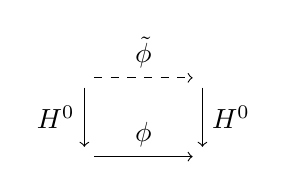
\begin{tikzpicture}[auto,->]
        \node (TwA) at (0,1) {$\Tw\A$}; 
        \node (TwB) at (1.5,1) {$\Tw\B$};
        \node (TrA) at (0,0) {$\Tr\A$}; 
        \node (TrB) at (1.5,0) {$\Tr\B$};
        \draw[dashed] (TwA) -- node {$\tilde{\phi}$} (TwB);
        \draw (TwA) -- node[swap] {$H^0$} (TrA);
        \draw (TwB) -- node {$H^0$} (TrB);
        \draw (TrA) -- node {$\phi$} (TrB);
        \end{tikzpicture}        
    \] 
  \end{question} 

  一般には, $\phi$のリフト$\tilde{\phi}$は存在しない. 

  \begin{example}
    $\A, \B$を次の条件を満たす極小$\Ainf$圏とする.
    \begin{itemize}
      \item $H(\A)$の$H(\B)$のいずれにおいても, 相異なる対象は同型でない. 
      \item 三角圏同値$\phi : \Tr\A \to \Tr\B$は存在する.
      \item 三角圏同値$\phi$の充満部分圏への制限$H(\A) \to H(\B)$は圏同型である.
    \end{itemize}
  $\A$と$\B$が$\Ainf$同型でないとき, $\phi$のリフト$\tilde{\phi} : \Tw\A \to \Tw\B$は存在しない.
  \end{example}
\end{frame}

% \begin{frame}{形式的な$\Ainf$圏}
%   $\Ainf$増強が一意であるような$\Ainf$圏の条件を考える. \\
%   まずは, 有理ホモトピー論で登場する(らしい)圏の条件を考える. 

%   \begin{definition}[形式的]
%     $\Ainf$圏$\A$がそのコホモロジー圏$H(\A)$(を$\Ainf$圏とみなしたもの)と$\Ainf$擬同型であるとき, $\A$は形式的(formal)であるという. 
%   \end{definition}

%   形式的な$\Ainf$圏に極小模型定理を用いると, $H(\A)$と$\Ainf$擬同型であることから, 微分と高次のホモトピーが自明な$\Ainf$圏を構成できる.
% \end{frame}

\begin{frame}{$\Ainf$増強が一意である$\Ainf$圏}
  $H(\A)$における射の合成を$2$次の$\Ainf$構造$\mu^2_\A$に持つ極小$\Ainf$圏$\A$がどのくらい存在するかを見る. 

  \begin{definition}[$\Ainf$拡張]
    次数付き圏$\B$における射の合成を$2$次の$\Ainf$構造に持つ極小$\Ainf$圏$\A$を$\B$の$\Ainf$拡張($\Ainf$-decoration of $\B$)という. 
  \end{definition}

  \begin{definition}[自明な$\Ainf$拡張]
    次数付き線形圏$H(\A)$の任意の$\Ainf$拡張が$H(\A)$と$\Ainf$擬同型
    \footnote{
      \cite{Kaj4}では$\Ainf$同型となっているが, おそらく$\Ainf$擬同型である(かもしれない).
    }
    であるとき, $H(\A)$の$\Ainf$拡張は自明である($\Ainf$-decoration of $H(\A)$ is trivial)という. 
  \end{definition}

  \begin{example}
    極小$\Ainf$圏$\A$が$H(\A) = H^0(\A)$を満たすとき, $\A$の$\Ainf$拡張は自明である. 
  \end{example} 

  $H(\A)$の$\Ainf$拡張が自明であるとき, $\Tr\A$の$\Ainf$増強は一意である. 

  \begin{theorem} \label{prop_trivial_Ainf_decoration_induces_unique_Ainf_enhancement}
    $\Ainf$圏$\A$の次数付き線形圏$H(\A)$の$\Ainf$拡張は自明であるとする. 
    このとき, 三角圏$\Tr\A$の$\Ainf$増強は$\Ainf$擬同値を除いて一意である. 
  \end{theorem}
\end{frame}

\begin{frame}{順序付き$\Ainf$圏}
  $\Ainf$拡張が自明である$\Ainf$圏として, 順序付き$\Ainf$圏がある. 

  \begin{definition}[順序付き]
    $\Ainf$圏$\A$の対象が有限個$X_1,\cdots,X_n$かつ, 任意の$1 \leq i,j \leq n$に対して$\hom_{H(\A)}(X_i,X_j)$が有限次元であり, 
    \begin{align*}
      \hom_{H(\A)}(X_i,X_j) =
      \begin{cases}
        \{\id_{X_i}\} & (i=j) \\
        \{0\} & (i>j)
      \end{cases}
    \end{align*}
    を満たすとき, $\A$は順序付き(directed)であるという. 
  \end{definition}

  $\A$が順序付き$\Ainf$圏のとき, $\Tr\A$における対象$(X_1,\cdots,X_n)$は例外的生成列をなす. 

  \begin{definition}[強順序付き]
    順序付き$\Ainf$圏$\A$が任意の$r \neq 0$に対して, $\hom^r_\A(X_i,X_j) = 0$を満たすとき, $\A$は強順序付き(strongly directed)であるという. 
  \end{definition}

  $\A$が強順序付き$\Ainf$圏のとき, $\Tr\A$における対象$(X_1,\cdots,X_n)$は強例外的生成列をなす.
\end{frame}

\begin{frame}{$\Tr\A$の持つ性質}
  強順序付き$\Ainf$圏$\A$に対して, $\Tr\A$は一意な$\Ainf$増強を持つ. 

  \begin{theorem}
    $\A$を強順序付き$\Ainf$圏とする.
    ここで, $\X := X_1 \oplus \cdots \oplus X_n, ~~ A := \hom^0_{\Tw\A}(\X,\X)$とおくと, 次の三角圏同値が存在する. 
    \begin{align*}
      \Tr\A \simeq D^b(\Mod\text{-}A)
    \end{align*}
    \footnote{
      $\Mod\text{-}A$は有限生成右$A$加群の有界導来圏である. 
    }
    特に, この$\Ainf$圏$\A$の$\Ainf$増強は$\Ainf$擬同値を除いて一意である. 
  \end{theorem}

  \begin{remark}
    上の対応は関手$\hom^0_{\Tw\A}(-,\X) : \Tr\A \to D^b(\Mod\text{-}A)$により与えられる. 
    特に, $X_i$は直規約射影$A$加群$P_i$にうつされる.
  \end{remark}
\end{frame}

\begin{frame}{最後に}
  三角圏が$\Ainf$増強を持つことと, 三角圏が代数的であることは同値である. 
  この命題は三角圏の$\Ainf$増強の存在性が三角圏の情報で与えられている.
  しかし, 三角圏の$\Ainf$増強の一意性は$\Ainf$拡張など$\Ainf$圏での情報で与えられており, 同値な命題も見つかっていない.
  \footnote{
    「準射影代数多様体の連接層の導来圏の増強は一意的である」ことを教えていただきました. 
  }
  \bigskip
  
  また, 個人的な意見として, 増強の具体的な構成はdg圏や$\Ainf$圏で考えるべきだと感じている. 
  しかし, $\Ainf$増強の一意性と同値な命題などの話は, $\Ainf$増強よりも$\infty$増強を考えて安定$\infty$圏の世界でみるべきだと思う. \bigskip

  次の2点はまだ勉強中です. 
  \begin{itemize}
    \item 増強としてのホモロジカルミラー対称性が示されている例があるのか.
    \item 三角圏としてはミラーであるが, $\Ainf$圏としてはミラーと呼べないような例はあるのか. 
  \end{itemize}
\end{frame}


\begin{frame}[allowframebreaks]{Reference}
  \scriptsize
  \beamertemplatetextbibitems
  \bibliographystyle{junsrt}
  \bibliography{A_infty_cf}
\end{frame}

\end{document}